\chapter{Analisi dei requisiti}
\label{cap:analisi-requisiti}

\intro{In questa sezione vengono analizzati i requisiti del progetto e ne viene data un'analisi ad alto livello, combinando una visione concettuale con una visione pratica ed implementativa. 
Vengono inoltre descritti i casi d'uso e i requisiti individuati, con l'obiettivo di fornire una visione generale del sistema e delle sue funzionalità, in modo semplice e comprensibile.}

\section{Descrizione ed analisi del sistema}
L'obiettivo del progetto è la creazione di una piattaforma per la visualizzazione di contenuti multimediali, in questo caso dei film,
tramite l'utilizzo degli standard \glsfirstoccur{\gls{w3cg}} \glsfirstoccur{\gls{didg}} e \glsfirstoccur{\gls{ssig}} per la verifica sicura dell'identità dell'utente e per la 
visualizzazione di tutti i contenuti della piattaforma, certificando in modo sicuro la propria identità senza diffondere dati personali tramite 
l'utilizzo di un \glsfirstoccur{\gls{zkpg}}.\\

Più precisamente, l'implementazione avviene usando lo \textit{smart contract} che implementa ad alto livello lo standard \glsfirstoccur{\gls{ssig}}, 
scritto nel linguaggio di programmazione \textit{Solidity} da parte dello studente magistrale Alessio De Biasi.
Questo contratto permette la gestione dell'identità digitale tramite la creazione di un documento di identità digitale, che contiene un identificatore univoco
chiamato \glsfirstoccur{\gls{didg}}, composto da una stringa alfanumerica che identifica l'utente, e un \textit{DID Document}, che contiene le informazioni dell'utente a lui associato.
Normalmente, la sua creazione avviene tramite un file \textit{json}, composto dallo standard di riferimento, l'identificativo ed un campo \textit{controller},
che ha la capacità di fare dei cambiamenti al documento stesso e certifica la firma digitale del documento, sulla base del metodo usato per la sua creazione.
Il formato del \textit{DID Document} è come il seguente (codice proveniente da \cite{site:didw3c}):

\begin{lstlisting}[language=json]
    {
      "@context": [
        "https://www.w3.org/ns/did/v1",
        "https://w3id.org/security/suites/ed25519-2020/v1"
      ]
      "id": "did:example:123456789abcdefghi",
      "authentication": [{    
        "id": "did:example:123456789abcdefghi#keys-1",
        "type": "Ed25519VerificationKey2020",
        "controller": "did:example:123456789abcdefghi",
        "publicKeyMultibase": "zH3C2AVvLMv6gmMNam3uVAjZpfkcJCwDwnZn6z3wXmqPV"
      }]
    }
\end{lstlisting}

\newpage

Nel codice che dovrà essere utilizzato come libreria,
ogni documento è caratterizzato da una \textit{capability delegation}, che permette di delegare l'accesso crittografico di un elemento ad un altro utente,
un servizio, specificando l'identificativo e l'indirizzo di un'entità autorizzata, un metodo di autenticazione, in cui viene stabilito
il modo in cui implementare il meccanismo di riconoscimento da parte dell'utente (dimostrando di fatto che sia chi dice di essere) e un 
genitore, composto da un identificativo ed una firma digitale.
L'idea del codice è di creare una cosiddetta `catena di fiducia', la cui idea è associare ad un utente un \glsfirstoccur{\gls{didg}} e dimostrare,
attraverso un meccanismo di autenticazione definito a priori nel documento tramite firme digitali, la risoluzione dei dati trasmessi, il riconoscimento univoco della sua identità
e l'accesso ad un determinato contenuto. Infatti, l'utente viene riconosciuto perché i suoi dati sono stati certificati da un ente 
con capacità di firma digitale che, a sua volta, si fida di altri enti anch'essi riconosciuti, fino ad arrivare ad un soggetto radice.
Se questa catena di fiducia viene risolta correttamente, l'utente viene riconosciuto univocamente e può accedere ai contenuti della piattaforma. \\

La struttura dati blockchain, attraverso l'utilizzo di un account associato ad un \glsfirstoccur{\gls{didg}}, permette di certificare l'identità dell'utente
tramite la firma digitale dei dati trasmessi con la propria coppia di chiavi pubblica/privata, certificando in modo immutabile la propria identità e
permette di realizzare un sistema di autenticazione sicuro e decentralizzato, che non richiede l'utilizzo di un ente terzo per la verifica delle informazioni. \\

L'utilizzo della piattaforma e delle sue parti prescinde dalla dimostrazione, attraverso una chiamata al contratto libreria fornito, della risoluzione attraverso firma digitale
del \glsfirstoccur{\gls{didg}} associato all'utente, che dimostra l'utilizzo di un account associato alla rete blockchain,
la sua identità. Se l'indirizzo che ha firmato digitalmente il documento è associato ad un profilo creatore di quel \glsfirstoccur{\gls{didg}} così firmato,
allora l'utente può accedere ai contenuti della piattaforma. L'implementazione di questo passaggio prevede che l'utente dimostri precisamente
la propria identità secondo un meccanismo \textit{challenge-response}: viene generato un numero casuale e viene chiesto all'utente di firmarlo digitalmente, in modo da dimostrare
che è in possesso della chiave privata associata all'indirizzo che ha firmato il documento. \\

Se il metodo di autenticazione conteneva la sua firma e come dato il numero casuale trasmesso, grazie alla generazione dell'identificatore
e la chiamata al contratto in grado di risalire precisamente all'account blockchain che l'ha emessa, si certifica l'utente in modo univoco.
Tale meccanismo viene implementato in fase di registrazione, in cui l'utente possiede un proprio \glsfirstoccur{\gls{didg}} e registra i propri dati anagrafici
e in fase di accesso, quando l'utente inserita esclusivamente come unico dato per effettuare il login il proprio identificatore, firmato digitalmente nella fase precedente e appartenente in modo univoco a lui. \\

In questa sezione, l'utente viene presentato ad un insieme di film e può scegliere di visualizzarne uno. Alla visualizzazione di un certo
contenuto oggetto a limiti di età, l'utente viene presentato ad una schermata di verifica, in cui deve dimostrare la sua età.
Questo passaggio avviene attraverso la creazione di una \glsfirstoccur{\gls{vpg}}, contenente molteplici \glsfirstoccur{\gls{vcg}}, 
con una associata all'utente (definito \textit{holder} delle credenziali) e le altre associate agli enti verificatori (definiti \textit{issuer}, che sono gli enti che hanno rilasciato le credenziali). \\

Normalmente, una \textit{Verifiable Presentation} è infatti composta da:
\begin{itemize}
    \item un insieme di metadati, che descrivono la presentazione;
    \item un insieme di \textit{Verifiable Credentials}, che sono le credenziali associate alla presentazione;
    \item un insieme di \textit{proof}, che sono le prove di autenticità delle credenziali.
\end{itemize}

Invece, una \textit{Verifiable Credential} è composta da:
\begin{itemize}
    \item un contesto di riferimento, che è un \textit{URI} che definisce il contesto di riferimento delle credenziali;
    \item un identificativo, che specifica il sito di riferimento;
    \item un tipo, che specifica se la credenziale è appropriata per la presentazione;
    \item un soggetto, che è l'identificativo dell'utente a cui sono associate le credenziali;
    \item un \textit{issuer}, che è l'identificativo dell'ente che ha rilasciato le credenziali;
    \item un \textit{issuanceDate}, che è la data di rilascio delle credenziali;
    \item una \textit{proof}, che è la prova di autenticità delle credenziali.
\end{itemize}

Il seguente è un esempio di una \textit{Verifiable Presentation} con al suo interno un insieme di \textit{Verifiable Credentials} (codice proveniente da \cite{site:vpw3c}):
\begin{lstlisting}[language=json]
    {
        "@context": [
          "https://www.w3.org/2018/credentials/v1",
          "https://www.w3.org/2018/credentials/examples/v1"
        ],
        "type": "VerifiablePresentation",
        "verifiableCredential": [
          {
            "@context": [
              "https://www.w3.org/2018/credentials/v1",
              "https://www.w3.org/2018/credentials/examples/v1"
            ],
            "type": ["VerifiableCredential", "UniversityDegreeCredential"],
            "credentialSchema": {
              "id": "did:example:cdf:35LB7w9ueWbagPL94T9bMLtyXDj9pX5o",
              "type": "did:example:schema:22KpkXgecryx9k7N6XN1QoN3gXwBkSU8SfyyYQG"
            },
            "issuer": "did:example:Wz4eUg7SetGfaUVCn8U9d62oDYrUJLuUtcy619",
            "credentialSubject": {
              "degreeType": "BachelorDegree",
              "degreeSchool": "College of Engineering"
            },
            "proof": {
              "type": "AnonCredDerivedCredentialv1",
              "primaryProof": "cg7wLNSi48K5qNyAVMwdYqVHSMv1Ur8i...Fg2ZvWF6zGvcSAsym2sgSk737",
              "nonRevocationProof": "mu6fg24MfJPU1HvSXsf3ybzKARib4WxG...RSce53M6UwQCxYshCuS3d2h"
            }
        }],
        "proof": {
          "type": "AnonCredPresentationProofv1",
          "proofValue": "DgYdYMUYHURJLD7xdnWRinqWCEY5u5fK...j915Lt3hMzLHoPiPQ9sSVfRrs1D"
        }
      }
\end{lstlisting}

Al suo interno, come si vede, sono presenti un insieme di credenziali, contenente un campo di dimostrazione di appartenenza ad uno schema comune,
a cui sarà associata la catena di fiducia, e degli insiemi di metodi di firma digitale, che dimostrano la validità delle credenziali presenti,
avendo ciascuna un insieme di \textit{issuer} riconosciuti. \\

Il meccanismo è in grado di integrarsi con \glsfirstoccur{\gls{zkpg}}, in cui la prova di appartenenza ad uno schema comune è dimostrata
senza rivelare informazioni sensibili di alcun tipo, combinando un insieme di \textit{Verifiable Credentials}, verificate tramite 
un insieme di \textit{issuer} riconosciuti dal sistema della catena di fiducia grazie all'uso della proprietà \textit{proof} descritta sopra
e la definizione di uno schema comune a cui fare riferimento, che certifica il riconoscimento in quanto firmato a catena da un insieme di \textit{issuer}
(secondo le specifiche dettagliate in \cite{site:zkpw3c}). \\
Questo permette all'utente di definire precisamente quali informazioni vuole rivelare e, attraverso l'utilizzo del contratto libreria, 
dimostrare la propria identità, verificato con questo meccanismo e accedendo al proprio contenuto di interesse. 

\section{Casi d'uso}

In questa sezione, saranno presenti un insieme di diagrammi dei casi d'uso, definiti secondo il linguaggio standard \glsfirstoccur{\gls{umlg}},
che descrivono le interazioni tra gli attori, definiti convenzionalmente come utenti del sistema e il sistema stesso. 
Seguirà una tabella di tracciamento dei requisiti, che mostrerà come i requisiti individuati nella sezione precedente siano soddisfatti
dai casi d'uso definiti in questa sezione, in base all'analisi prevista. \\

Di seguito, un diagramma complessivo (in figura \ref{fig:usecase-scenario-principale}) dei casi d'uso individuati, che verranno descritti nel dettaglio successivamente:

\begin{figure}[!h] 
    \centering 
    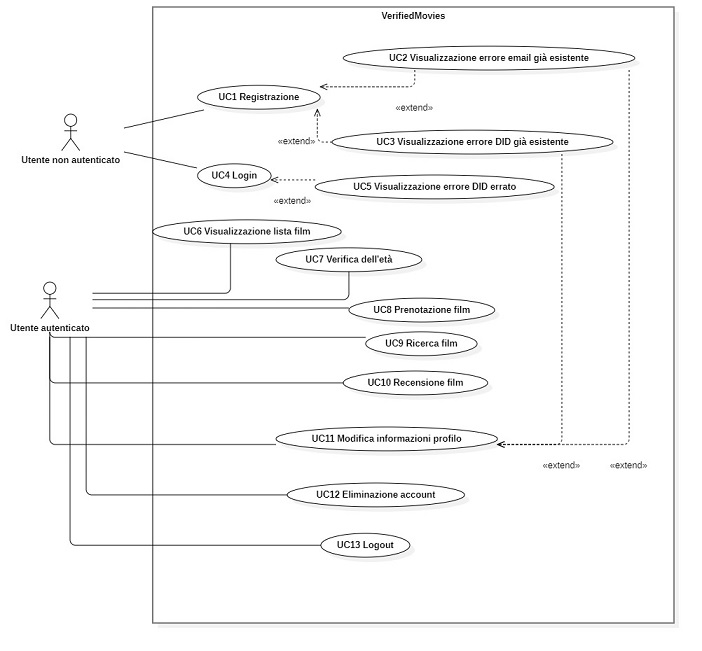
\includegraphics[width=0.9\columnwidth, alt={Scenario principale dei vari casi d'uso individuati}]{immagini/usecase/scenario-principale.jpg}
    \caption{Scenario principale}\label{fig:usecase-scenario-principale}
\end{figure}

\begin{usecase}{1}{Registrazione}\label{uc:registrazione}
\usecaseactors{Utente non autenticato}
\usecasepre{L'utente ha avviato l'applicazione web e ha aperto la pagina di registrazione}
\usecasedesc{L'utente vuole registrarsi presso l'applicazione web}
\usecasepost{L'utente ha completato la registrazione e può effettuare il login}
\usecasemain{L'utente: }

\begin{enumerate}
  \item inserisce il proprio username (UC1.1);
  \item inserisce la propria email (UC1.2);
  \item inserisce il proprio DID (UC1.3);
  \item inserisce la propria data di nascita (UC1.4).
\end{enumerate}

\usecaseext{}
\begin{enumerate}
  \item Visualizzazione errore email già esistente (UC2);
  \item Visualizzazione errore DID già esistente (UC3).
\end{enumerate}
\end{usecase}

\begin{figure}[!h] 
  \centering 
  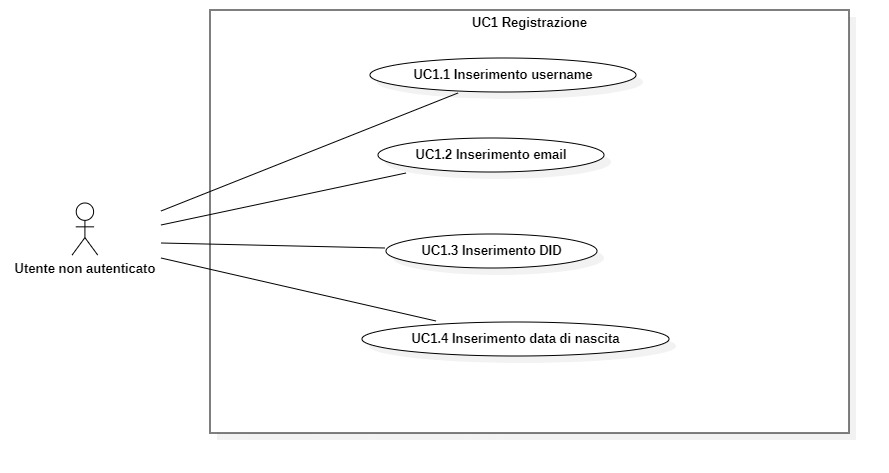
\includegraphics[width=0.9\columnwidth, alt={Caso d'uso relativo alla registrazione}]{immagini/usecase/UC1.jpg}
  \caption{UC1: Registrazione}\label{fig:uc:registrazione}
\end{figure}

\begin{usecase}{1.1}{Inserimento username}\label{uc:registrazione-username}
  \usecaseactors{Utente non autenticato}
  \usecasepre{L'utente ha avviato l'applicazione web e ha aperto la pagina di registrazione}
  \usecasedesc{L'utente deve inserire uno username per registrarsi presso l'applicazione web}
  \usecasepost{L'utente ha inserito lo username e può procedere con la registrazione}
  \usecasemain{}
  
  \begin{enumerate}
    \item L'utente inserisce il proprio username.
  \end{enumerate}
  
\end{usecase}

\begin{usecase}{1.2}{Inserimento email}\label{uc:registrazione-email}
  \usecaseactors{Utente non autenticato}
  \usecasepre{L'utente ha avviato l'applicazione web e ha aperto la pagina di registrazione}
  \usecasedesc{L'utente deve inserire una email per registrarsi presso l'applicazione web}
  \usecasepost{L'utente ha inserito la propria mail e può procedere con la registrazione}
  \usecasemain{}
  
  \begin{enumerate}
    \item L'utente inserisce la propria email.
  \end{enumerate}
  
\end{usecase}

\begin{usecase}{1.3}{Inserimento DID}\label{uc:registrazione-did}
  \usecaseactors{Utente non autenticato}
  \usecasepre{L'utente ha avviato l'applicazione web e ha aperto la pagina di registrazione}
  \usecasedesc{L'utente deve inserire il proprio DID per registrarsi presso l'applicazione web}
  \usecasepost{L'utente ha inserito il proprio DID e può procedere con la registrazione}
  \usecasemain{}
  
  \begin{enumerate}
    \item L'utente inserisce il proprio DID.
  \end{enumerate}
  
\end{usecase}

\begin{usecase}{1.4}{Inserimento data di nascita}\label{uc:registrazione-data}
  \usecaseactors{Utente non autenticato}
  \usecasepre{L'utente ha avviato l'applicazione web, non è autenticato e ha aperto la pagina di registrazione}
  \usecasedesc{L'utente deve inserire la propria data di nascita per registrarsi presso l'applicazione web}
  \usecasepost{L'utente ha inserito la propria data di nascita e può procedere con la registrazione}
  \usecasemain{}
  
  \begin{enumerate}
    \item L'utente inserisce la propria data di nascita.
  \end{enumerate}
  
\end{usecase}

\begin{usecase}{2}{Visualizzazione errore email già esistente}\label{uc:registrazione-email-esistente}
  \usecaseactors{Utente non autenticato}
  \usecasepre{L'utente ha inserito una email già esistente}
  \usecasedesc{L'utente deve inserire una email diversa per registrarsi presso l'applicazione web}
  \usecasepost{L'utente ha inserito una email diversa e può procedere con la registrazione}
  \usecasemain{}
  
  \begin{enumerate}
    \item L'utente visualizza un messaggio di errore che lo informa che la email inserita è già presente nel sistema.
  \end{enumerate}
\end{usecase}

\begin{usecase}{3}{Visualizzazione errore DID già esistente}\label{uc:registrazione-did-esistente}
  \usecaseactors{Utente non autenticato}
  \usecasepre{L'utente ha inserito un DID già esistente}
  \usecasedesc{L'utente deve inserire un DID diverso per registrarsi presso l'applicazione web}
  \usecasepost{L'utente ha inserito un DID diverso e può procedere con la registrazione}
  \usecasemain{}
  
  \begin{enumerate}
    \item L'utente visualizza un messaggio di errore che lo informa che il DID inserito è già presente nel sistema.
  \end{enumerate}
\end{usecase}

\begin{usecase}{4}{Login}\label{uc:autenticazione}
  \usecaseactors{Utente non autenticato}
  \usecasepre{L'utente ha avviato l'applicazione web, non è già autenticato e ha aperto la pagina di autenticazione}
  \usecasedesc{L'utente vuole entrare presso il sito e deve inserire le proprie credenziali per autenticarsi}
  \usecasepost{L'utente è autenticato correttamente e può procedere con l'utilizzo dell'applicazione}
  \usecasemain{}
  
  \begin{enumerate}
    \item L'utente inserisce il proprio DID.
  \end{enumerate}

  \usecaseext{}
  \begin{enumerate}
    \item Visualizzazione errore DID errato (UC5).
  \end{enumerate}
\end{usecase}

\begin{figure}[!h] 
  \centering 
  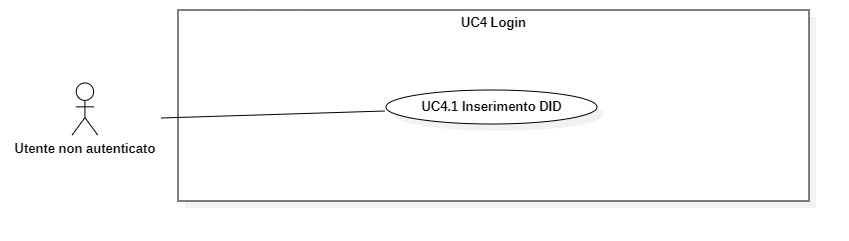
\includegraphics[width=0.9\columnwidth, alt={Caso d'uso relativo all'autenticazione dell'utente}]{immagini/usecase/UC4.jpg}
  \caption{UC4: Login}\label{fig:uc:autenticazione}
\end{figure}

\begin{usecase}{4.1}{Inserimento DID}\label{uc:autenticazione-did}
  \usecaseactors{Utente non autenticato}
  \usecasepre{L'utente ha avviato l'applicazione web, non è già autenticato e ha aperto la pagina di autenticazione}
  \usecasedesc{L'utente deve inserire il proprio DID associato alle proprie credenziali per autenticarsi presso l'applicazione web}
  \usecasepost{L'utente ha inserito il proprio DID e può procedere con l'autenticazione}
  \usecasemain{}
  
  \begin{enumerate}
    \item L'utente inserisce il proprio DID.
  \end{enumerate}

\end{usecase}

\begin{usecase}{5}{Visualizzazione lista film}\label{uc:visualizzazione-lista-film}
  \usecaseactors{Utente autenticato}
  \usecasepre{L'utente è autenticato e ha aperto la pagina principale dell'applicazione web}
  \usecasedesc{L'utente vuole visualizzare la lista dei film presenti nel sistema}
  \usecasepost{L'utente ha visualizzato la lista dei film presenti nel sistema}
  \usecasemain{}
  
  \begin{enumerate}
    \item L'utente visualizza la lista dei film presenti nel sistema.
  \end{enumerate}
\end{usecase}

\begin{figure}[!h] 
  \centering 
  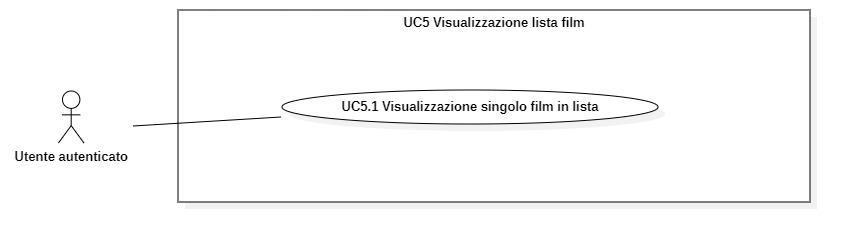
\includegraphics[width=0.9\columnwidth, alt={Caso d'uso relativo alla visualizzazione della lista dei film dell'utente}]{immagini/usecase/UC5.jpg}
  \caption{UC5: Visualizzazione lista film}\label{fig:uc:visualizzazione-lista-film}
\end{figure}

\begin{usecase}{5.1}{Visualizzazione singolo film in lista}\label{uc:visualizzazione-singolo-lista-film}
  \usecaseactors{Utente autenticato}
  \usecasepre{L'utente è autenticato e ha aperto la pagina principale dell'applicazione web}
  \usecasedesc{L'utente vuole visualizzare un singolo film dalla lista dei film presenti nel sistema}
  \usecasepost{L'utente ha visualizzato un film tra la lista di quelli presenti nel sistema}
  \usecasemain{}
  
  \begin{enumerate}
    \item L'utente visualizza un film tra quelli presenti nella lista del sistema.
  \end{enumerate}
\end{usecase}

\begin{usecase}{6}{Verifica dell'età}\label{uc:verifica-eta}
  \usecaseactors{Utente autenticato}
  \usecasepre{L'utente è autenticato, possiede una Verifiable Credential che attesta la sua età e intende visualizzare un film per prenotarlo} 
  \usecasedesc{L'utente vuole visualizzare un singolo film dalla lista dei film presenti nel sistema}
  \usecasepost{L'utente ha verificato la propria età in modo sicuro e può procedere con la prenotazione del film in oggetto}
  \usecasemain{}
  
  \begin{enumerate}
    \item L'utente seleziona un film dalla lista dei film presenti nel sistema;
    \item Il sistema prende la categoria di età del film selezionato e la confronta con l'età dell'utente.
    \item L'utente presenta la propria Verifiable Credential che attesta la sua età.
    \item Il sistema verifica la correttezza della Verifiable Credential utilizzando il DID del soggetto che l'ha rilasciata e genera una Verifiable Presentation contenente una Zero Knowledge Proof.
    \item Il sistema verifica la validità della Zero Knowledge Proof e verifica che l'età dell'utente sia maggiore o uguale a quella del film.
    \item Se la verifica ha successo, l'utente può procedere con la prenotazione del film.
  \end{enumerate}
\end{usecase}

\begin{usecase}{7}{Prenotazione film}\label{uc:prenotazione-film}
  \usecaseactors{Utente autenticato}
  \usecasepre{L'utente è autenticato, ha verificato la propria età e ha selezionato un film dalla lista dei film presenti nel sistema}
  \usecasedesc{L'utente vuole prenotare il film che ha selezionato dalla lista dei film presenti nel sistema}
  \usecasepost{L'utente ha verificato la propria età in modo sicuro e il film che ha selezionato è stato prenotato}
  \usecasemain{}
  
  \begin{enumerate}
    \item L'utente seleziona un film dalla lista dei film presenti nel sistema;
    \item Il sistema richiede all'utente di fornire i dettagli della prenotazione; 
    \item L'utente inserisce la data di prenotazione (UC7.1), l'orario di prenotazione (UC7.2) e il numero di posti da prenotare (UC7.3);
    \item Il sistema verifica la disponibilità del film per la data e l'orario selezionati e registra l'avvenuta prenotazione, fornendo un riepilogo all'utente.
  \end{enumerate}
\end{usecase}

\begin{figure}[!h] 
  \centering 
  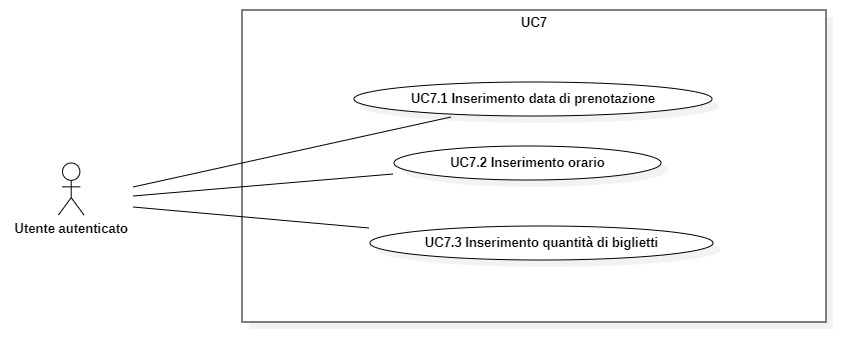
\includegraphics[width=0.9\columnwidth, alt={Caso d'uso relativo alla prenotazione di un film dell'utente}]{immagini/usecase/UC7.jpg}
  \caption{UC7: Prenotazione film}\label{fig:uc:prenotazione-film}
\end{figure}

\begin{usecase}{7.1}{Inserimento data prenotazione}\label{uc:inserimento-data-prenotazione}
  \usecaseactors{Utente autenticato}
  \usecasepre{L'utente è autenticato, ha verificato la propria età e ha selezionato un film dalla lista dei film presenti nel sistema}
  \usecasedesc{L'utente vuole inserire la data di prenotazione del film che ha selezionato dalla lista dei film presenti nel sistema}
  \usecasepost{L'utente ha inserito la data di prenotazione}
  \usecasemain{}
  
  \begin{enumerate}
    \item L'utente inserisce la data di prenotazione per il film che intende prenotare.
  \end{enumerate}
\end{usecase}

\begin{usecase}{7.2}{Inserimento orario prenotazione}\label{uc:inserimento-orario-prenotazione}
  \usecaseactors{Utente autenticato}
  \usecasepre{L'utente è autenticato, ha verificato la propria età e ha selezionato un film dalla lista dei film presenti nel sistema}
  \usecasedesc{L'utente vuole inserire l'orario di prenotazione del film che ha selezionato dalla lista dei film presenti nel sistema}
  \usecasepost{L'utente ha inserito l'orario di prenotazione}
  \usecasemain{}
  
  \begin{enumerate}
    \item L'utente inserisce l'orario di prenotazione per il film che intende prenotare.
  \end{enumerate}
\end{usecase}

\begin{usecase}{7.3}{Inserimento numero posti}\label{uc:inserimento-numero-posti}
  \usecaseactors{Utente autenticato}
  \usecasepre{L'utente è autenticato, ha verificato la propria età e ha selezionato un film dalla lista dei film presenti nel sistema}
  \usecasedesc{L'utente vuole inserire il numero di posti da prenotare per il film che ha selezionato dalla lista dei film presenti nel sistema}
  \usecasepost{L'utente ha inserito il numero di posti da prenotare}
  \usecasemain{}
  
  \begin{enumerate}
    \item L'utente inserisce il numero di posti da prenotare per il film che intende prenotare.
\end{enumerate}
\end{usecase}

\begin{usecase}{8}{Ricerca film}\label{uc:ricerca-film}
  \usecaseactors{Utente autenticato}
  \usecasepre{L'utente è autenticato}
  \usecasedesc{L'utente vuole cercare un film presente nel sistema e nel sistema sono presenti dei film}
  \usecasepost{L'utente ha cercato un film presente nel sistema e il sistema ha restituito i risultati della ricerca, permettendo all'utente di interagire con essi}
  \usecasemain{}
  
  \begin{enumerate}
    \item L'utente accede alla pagina principale contenente la lista dei film presenti nel sistema;
    \item L'utente inserisce il titolo del film che vuole cercare;
    \item Il sistema ricerca il film all'interno del sistema e restituisce i risultati della ricerca all'utente.
  \end{enumerate}
\end{usecase}

\begin{usecase}{9}{Recensione film}\label{uc:recensione-film}
  \usecaseactors{Utente autenticato}
  \usecasepre{L'utente è autenticato e visualizza la lista dei film prenotati}
  \usecasedesc{L'utente vuole recensire un film presente nel sistema}
  \usecasepost{L'utente ha recensito correttamente un film tra quelli presenti, anche senza prenotazione}
  \usecasemain{}
  
  \begin{enumerate}
    \item L'utente accede alla pagina principale contenente la lista dei film prenotati;
    \item L'utente seleziona il film che vuole recensire;
    \item L'utente inserisce la recensione del film;
    \item Il sistema registra la recensione del film e la associa all'utente che l'ha inserita.
  \end{enumerate}
\end{usecase}

\begin{usecase}{10}{Modifica informazioni profilo}\label{uc:modifica-informazioni-account}
  \usecaseactors{Utente autenticato}
  \usecasepre{L'utente è autenticato}
  \usecasedesc{L'utente vuole modificare le proprie informazioni personali}
  \usecasepost{L'utente ha modificato le proprie informazioni personali di proprio interesse}
  \usecasemain{}
  
  \begin{enumerate}
    \item L'utente accede alla pagina principale contenente le proprie informazioni personali;
    \item L'utente modifica il proprio username (UC10.1);
    \item L'utente modifica la propria email (UC10.2);
    \item L'utente modifica il proprio DID (UC10.3);
    \item L'utente modifica la propria data di nascita (UC10.4);
  \end{enumerate}

  \usecaseext{}
  \begin{enumerate}
    \item Visualizzazione errore email già esistente (UC2);
    \item Visualizzazione errore DID già esistente (UC3).
  \end{enumerate}
\end{usecase}

\begin{figure}[!h] 
  \centering 
  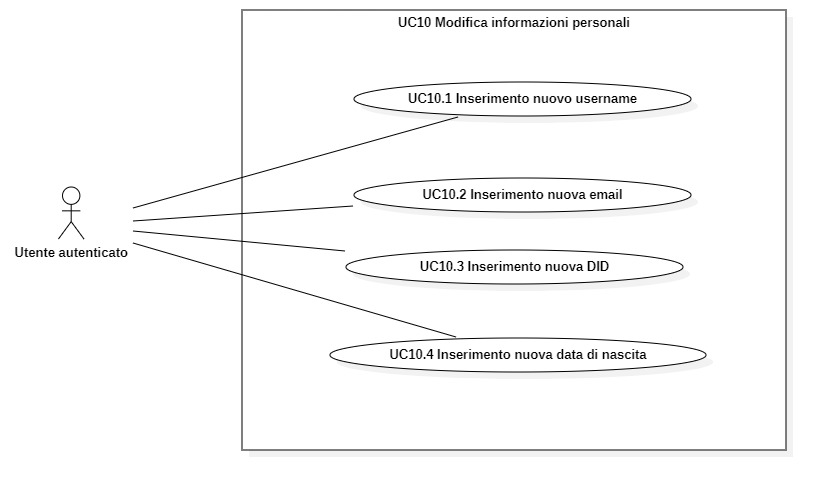
\includegraphics[width=0.9\columnwidth, alt={Caso d'uso relativo alla modifica delle informazioni del profilo}]{immagini/usecase/UC10.jpg}
  \caption{UC10: Modifica informazioni profilo}\label{fig:uc:prenotazione-film}
\end{figure}

\begin{usecase}{10.1}{Inserimento nuovo username}\label{uc:modifica-username}
  \usecaseactors{Utente autenticato}
  \usecasepre{L'utente è autenticato e intende modificare il proprio username}
  \usecasedesc{L'utente vuole modificare lo username associato al proprio account}
  \usecasepost{L'utente ha inserito il proprio username correttamente}
  \usecasemain{}
  
  \begin{enumerate}
    \item L'utente modifica il proprio username e conferma l'operazione.
  \end{enumerate}
  
\end{usecase}

\begin{usecase}{10.2}{Inserimento nuova email}\label{uc:modifica-email}
  \usecaseactors{Utente autenticato}
  \usecasepre{L'utente è autenticato e intende modificare la propria email}
  \usecasedesc{L'utente vuole modificare la mail associata al proprio account}
  \usecasepost{L'utente ha modificato la propria email correttamente}
  \usecasemain{}
  
  \begin{enumerate}
    \item L'utente modifica la propria email e conferma l'operazione.
  \end{enumerate}
  
\end{usecase}

\begin{usecase}{10.3}{Inserimento nuova data di nascita}\label{uc:modifica-data-nascita}
  \usecaseactors{Utente autenticato}
  \usecasepre{L'utente è autenticato e intende modificare la propria data di nascita}
  \usecasedesc{L'utente vuole modificare la data di nascita associata al proprio account}
  \usecasepost{L'utente ha modificato la data di nascita correttamente}
  \usecasemain{}
  
  \begin{enumerate}
    \item L'utente modifica la propria data di nascita e conferma l'operazione.
  \end{enumerate}
  
\end{usecase}

\begin{usecase}{11}{Eliminazione account}\label{uc:eliminazione-account}
  \usecaseactors{Utente autenticato}
  \usecasepre{L'utente è autenticato e intende eliminare il proprio account}
  \usecasedesc{L'utente vuole eliminare il proprio account dal sistema}
  \usecasepost{L'utente ha eliminato il proprio account e il sistema ha eliminato tutti i dati ad esso associati}
  \usecasemain{}
  
  \begin{enumerate}
    \item L'utente accede alla pagina principale contenente di modifica del profilo contenente le proprie informazioni personali;
    \item L'utente elimina il proprio account;
    \item Il sistema elimina l'account dell'utente, cancellando il DID e le informazioni ad esso associate.
  \end{enumerate}
\end{usecase}

\begin{usecase}{12}{Logout}\label{uc:logout}
  \usecaseactors{Utente autenticato}
  \usecasepre{L'utente è autenticato e intende uscire dalla propria sessione}
  \usecasedesc{L'utente vuole effettuare il logout dal sistema}
  \usecasepost{L'utente ha effettuato il logout e il sistema ha terminato la sessione dell'utente, non permettendo più l'accesso alle funzionalità riservate}
  \usecasemain{}
  
  \begin{enumerate}
    \item L'utente accede alla pagina principale contenente le proprie informazioni personali;
    \item L'utente effettua il logout;
    \item Il sistema effettua il logout dell'utente e l'utente è uscito dalla propria sessione.
  \end{enumerate}
\end{usecase}

\section{Tracciamento dei requisiti}

Da un'attenta analisi dei requisiti e degli use case effettuata sul progetto è stata stilata la tabella che traccia i requisiti in rapporto agli use case.\\
Sono stati individuati diversi tipi di requisiti e si è quindi fatto utilizzo di un codice identificativo per distinguerli.\\
Il codice dei requisiti è così strutturato R(F/Q/V)(N/D/O) dove:
\begin{enumerate}
	\item[R =] requisito
    \item[F =] funzionale
    \item[Q =] qualitativo
    \item[V =] di vincolo
    \item[N =] obbligatorio (necessario)
    \item[D =] desiderabile
    \item[Z =] opzionale
\end{enumerate}

Le fonti dei requisiti sono:
\begin{itemize}
  \item \textbf{UC} = use case
  \item \textbf{Interno} = requisito individuato dall'insieme di stagisti e tutor aziendali
\end{itemize}

Nelle tabelle \ref{tab:requisiti-funzionali}, \ref{tab:requisiti-qualitativi} e \ref{tab:requisiti-vincolo} sono riassunti i requisiti e il loro tracciamento con gli use case delineati in fase di analisi.

\newpage

\begin{table}%
\caption{Tabella del tracciamento dei requisiti funzionali}
\label{tab:requisiti-funzionali}
\begin{tabularx}{\textwidth}{lXl}
\hline\hline
\textbf{Requisito} & \textbf{Descrizione} & \textbf{Use Case}\\
\hline
RFN-1     & L'interfaccia permette di configurare il tipo di sonde del test & UC1 \\
\hline
\end{tabularx}
\end{table}%

\begin{table}%
\caption{Tabella del tracciamento dei requisiti qualitativi}
\label{tab:requisiti-qualitativi}
\begin{tabularx}{\textwidth}{lXl}
\hline\hline
\textbf{Requisito} & \textbf{Descrizione} & \textbf{Use Case}\\
\hline
RQD-1    & Le prestazioni del simulatore hardware deve garantire la giusta esecuzione dei test e non la generazione di falsi negativi & - \\
\hline
\end{tabularx}
\end{table}%

\begin{table}%
\caption{Tabella del tracciamento dei requisiti di vincolo}
\label{tab:requisiti-vincolo}
\begin{tabularx}{\textwidth}{lXl}
\hline\hline
\textbf{Requisito} & \textbf{Descrizione} & \textbf{Use Case}\\
\hline
RVO-1    & La libreria per l'esecuzione dei test automatici deve essere riutilizzabile & - \\
\hline
\end{tabularx}
\end{table}%
